\documentclass[tikz,border=10pt]{standalone}
\usetikzlibrary{angles,quotes,calc}

\begin{document}
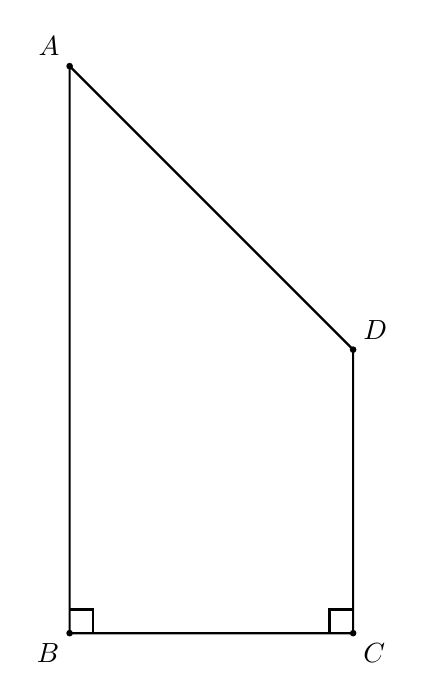
\begin{tikzpicture}[scale=1.2, thick]
    % 1. 定义坐标
    \coordinate (B) at (0,0);
    \coordinate (C) at (3,0);
    \coordinate (D) at (3,3);
    \coordinate (A) at (0,6);

    % 2. 绘制多边形边框
    \draw (A) -- (B) -- (C) -- (D) -- cycle;

    % 3. 标注顶点 (使用 node 命令)
    \node[above left] at (A) {$A$};
    \node[below left] at (B) {$B$};
    \node[below right] at (C) {$C$};
    \node[above right] at (D) {$D$};

    % 4. 绘制直角标记
    % 定义直角边长度
    \def\marksize{0.25}
    \draw (B) ++(\marksize,0) -- ++(0,\marksize) -- ++(-\marksize,0);
    \draw (C) ++(-\marksize,0) -- ++(0,\marksize) -- ++(\marksize,0);

    % 5. 可选：绘制顶点处的点
    \foreach \p in {A,B,C,D}
        \fill (\p) circle (1pt);

\end{tikzpicture}
\end{document}